\chapter[Detection of Cosmic-Rays and Extensive Air Showers]{\centering Detections of Cosmic-Rays \\ and Extensive Air Showers \\}\label{Ch:CR_Detection}

\section{Extensive Air Showers}

Use Earth's atmosphere as an interaction medium.
Primary particle interacts with the molecules in the atmosphere to produce a cascade of secondary particles. This cascade of particles is referred to as an Extensive Air Shower (EAS).
Hadronic primaries can produce pions, muons and other stuff.
Mixture of a hadronic core with an electromagnetic component from the decay of $\pi^{0}$.

Shower profile has particles produced until energy on individual secondary particles drop below the ionization threshold. Therefore the shower will reach a point of maximum particle number then will drop off.

\begin{figure}
\centering
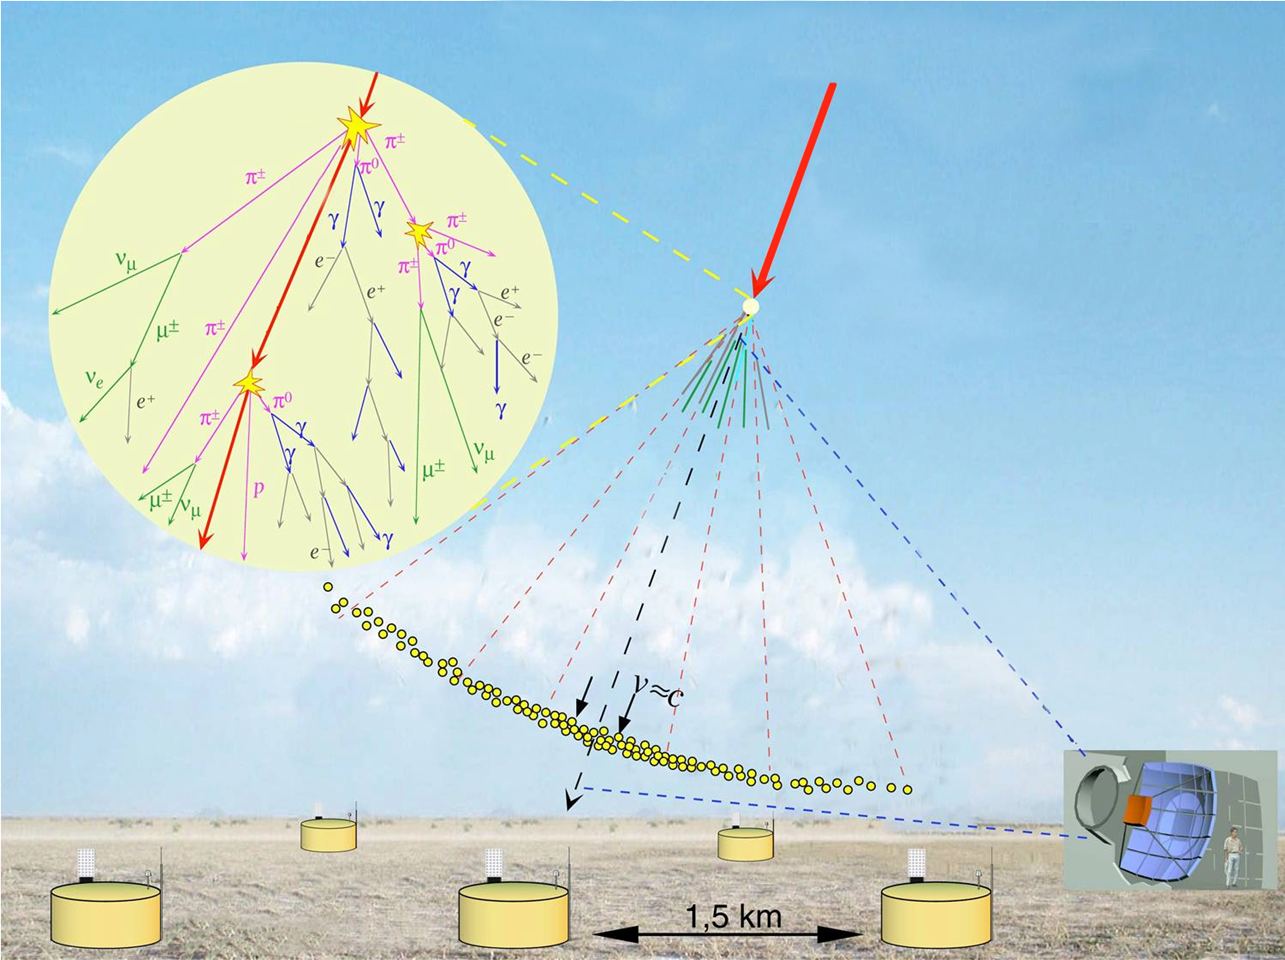
\includegraphics[width=0.7\textwidth]{chapters/pix/CR_ExtensiveAirShowers.png}
\caption{Diagram of Cosmic-ray Extensive Air Showers.}
\end{figure}

\section{Fluorescence Production}

The charge particles of EAS interact with the nitrogen molecules in the atmosphere. This interaction turns the nitrogen molecule dipole like and when the nitrogen returns to a ground state, a photon is emitted. This emitted photon is termed fluorescence light. Fluorescence light is can be emitted isotropically and typically in the UV band (between 300 and 400 nm). *** Show wavelength profile ***


\section{Atmospheric Effects}




\section{Detectors and History}

Early Experiments:

Volcano Ranch

Haverah Park

SUGAR

Yakutsk array is located in Russia and has been operating in different forms since 1967. The array reached a maximum collecting area of 17 km$^2$ around 1990. Recently it has been reconfigured to have a collection area of 8 km$^2$ to study lower energy cosmic-rays.

Akeno Gaint Air Shower Array (AGASA) is located in Tokyo, Japan. Operating at an average altitude of 667 m above sea level from 1990 to 2004. The array consist of over one hundred scintillator detectors covering 100 km$^2$ ***check this***. The timing measurements and data collection is achieved via interconnected optical fibers.

The Fly's Eye was the first successful air fluorescence detector operating from 1981 to 1993 at the Dugway Proving Grounds in Utah, USA. Fly's Eye achieved a time averaged aperture of about 100 km$^2$sr at the highest energies, considering it only operated on clear moonless nights. 

HiRes improved on the Fly's Eye design by advancing resolution and sensitivity, This was achieved by increasing the telescope effective mirror area to 3.8 m$^2$ and reducing the camera pixel angular diameter to 1\textdegree. 